\documentclass[a4paper,oneside]{memoir}
\usepackage[hidelinks]{hyperref}
\usepackage[utf8]{inputenc}
\usepackage{amssymb}
\usepackage{graphicx}
\usepackage{amsmath}
%\usepackage{epstopdf}
\usepackage{amsthm}
\usepackage{xcolor}
\usepackage{cleveref}
\usepackage{ifthen}
\usepackage{thmtools}
\usepackage{acronym}
\usepackage{cancel}

\renewcommand{\subsection}[1]{
\noindent\textbf{#1}\newline}
\pagestyle{ruled}

\title{Notes on Information Theory}
\author{Cristian Di Pietrantonio \and Michele Laurenti}


\newtheorem{prop}{Proposition}
\newtheorem{definition}{Definition}
\newtheorem{thm}{Theorem}
\newtheorem{obs}{Observation}
\newtheorem{lem}{Lemma}
\newtheorem{cor}{Corollary}

% math symbols

\newcommand{\M}{\mathcal{M}}
\newcommand{\X}{\mathcal{X}}
\newcommand{\Y}{\mathcal{Y}}

\newcommand{\Tau}{\mathrm{T}} % Capital Tau

\newcommand{\ie}{\textit{i.e.}, }

\newcommand{\xset}{\X}
\newcommand{\msgset}{\M} % the set of all messages
\newcommand{\yset}{\Y}
\newcommand{\cwset}{\mathcal{C}_n} % codewords set

\newcommand{\chrom}[1]{X(#1)}

\newcommand{\str}[1]{\underline{#1}} % string/vector
\newcommand{\zero}{\str{0}} % zero vector

\newcommand{\Reals}{\mathbb{R}}
\newcommand{\Naturals}{\mathbb{N}}

\newcommand{\abs}[1]{\left|{#1}\right|}
\newcommand{\floor}[1]{\left\lfloor{#1}\right\rfloor}
\newcommand{\ceil}[1]{\left\lceil{#1}\right\rceil}

\newcommand{\im}{\text{Im}} % image of linear application

\newcommand{\sfrac}{\frac}
\newcommand{\ifrac}[2]{\frac{#1}{#2}} % Inline fraction

\newcommand{\hball}[2]{B_H\left(#1, #2\right)} % the Hamming ball
\newcommand{\hdist}[1]{d_H \left({#1}\right)} % Hamming distance
\newcommand{\hweight}[1]{w_H\left(#1\right)} % Hamming weight

\renewcommand{\pref}{\leftarrowtail} % is prefix relation
\newcommand{\prol}[1]{Y_L(#1)} % all the strings that have x as prefix

\newcommand{\supp}{\text{Supp}_w} % support


\makeatletter
\renewcommand\thmt@mklistcmd{%
  \@xa\protected@edef\csname l@\thmt@envname\endcsname{% CHECK: why p@edef?
    \@nx\@dottedtocline{1}{1.5em}{\@nx\thmt@listnumwidth}{\thmt@thmname}{mu}%
  }%
  \ifthmt@isstarred
    \@xa\def\csname ll@\thmt@envname\endcsname{%
      \protect\numberline{\thmt@thmname\protect\let\protect\autodot\protect:}%
      \ifx\@empty\thmt@shortoptarg\else\protect\thmtformatoptarg{\thmt@shortoptarg}\fi
    }%
  \else
    \@xa\def\csname ll@\thmt@envname\endcsname{%
      % \thmt@thmname\ \csname the\thmt@envname\endcsname: \hfil%
      \ifx\@empty\thmt@shortoptarg\else\thmt@shortoptarg\fi
    }%
  \fi
  \@xa\gdef\csname thmt@contentsline@\thmt@envname\endcsname{%
    \thmt@contentslineShow% default:show
  }%
}
\makeatother


\begin{document}
	\frontmatter

	\maketitle
	\clearpage

	\tableofcontents*

	\mainmatter

	\chapter{Introduction}
Information Theory is born from one man, Cloude Shannon (1926 - 2001). It has to do with probability, algebra, coding theory, ergodic theory and appears in daily life. 

\begin{itemize}
	\item Tom Cover, Joy Thomas, Information Theory, Wiley;
	\item IT: cooling theorems for discrete memoryless systems, Korner;
	\item IT, Robert Ash.
\end{itemize}

%In communication you want to be understood, but you also want to avoid redundancy and words tend to be lengthy; there is a conflict of interest. Why some words are short and others are long? Short words encode common abstract pictures whereas long words must carry the whole information not available in common knowledge. Suggested readings: 

%\section{Base concepts and considerations}
%Define $\msgset$ as the finite set of all messages over an alphabet $\Sigma$. A message $m$ is an element of $\msgset$. Hartley, who introduced this concept before Shannon, stated that the maximum amount of information is equal to $\log_2 |\msgset|$, since one can identify elements of $\msgset$ with binary strings of length $\log_2 |\msgset|$. Formally $$\msgset \sim \{0, 1\}^{\left\lceil\log_2 |\msgset|\right\rceil} $$ and $$ m \sim \Delta \in \{0, 1\}^{\left\lceil\log_2 |\msgset|\right\rceil}.$$

%One can think of $\Delta$ as a sequence of $\log_2 |\msgset|$ binary questions that identify an element in $\msgset$. A single unit of information is a $0$ or $1$ (Binary Information Theory). In the \emph{20 question game}, where you need to minimize the number of questions to guess what a person thinks, is given a probability distribution $P$ over $\msgset$ (denoted from now on as $P|M$) s.t. $P(m) \geq 0,\ \forall m \in \msgset$ and $\sum_{m \in \msgset} P(m) = 1$. The questions can be designed to make the game as short as possible if $P$ is known.

%Must be noted that $|\underline{x}| = i \Leftrightarrow \underline{x} \in \{0, 1\}^{i}$. The number of questions asked on average must be minimized. Let $f: \msgset \rightarrow \{0, 1\}^*$, in other words a mapping from the message set to the sequences of answers to find the message then we want to minimize 
%\begin{equation} \label{eq:problen}
%\sum_{m \in \msgset} P(m) |f(m)|.
%\end{equation} 
%This equation is tied only to the probability distribution, not to the set or the questions. If $P$ is uniform then the Expression \ref{eq:problen} is equal to $\left\lceil\log_2 |\msgset|\right\rceil$. The function $f$ is called \emph{code}. The code is not always invertible.

%Communication happens at a distance, otherwise it would be trivial. There is some device that makes communication possible; the channel is not perfect. The noise is random, modeled through a probability distribution. The information source is not predictable either and will have its own probability distribution too. Encoding and decoding must be optimized to make communications short to reduce loss of information, and to reliably transmit, i.e. the receiver is reasonably sure that it gets what was sent. The two aspects are in contrast, you need and optimal trade-off. Usually partners in communication are separated in space and communication takes place in time. Sometimes in computer science the opposite thing happens: communication is storing information in space to retrieve it later in time. Sometimes you want to shorten the communication time, sometimes the space communication takes.
	%October 2016, the 4th
\chapter{The Hamming Ball}

This Chapter introduces an important concept: the Hamming Ball.

\section{Hamming space}

A \emph{space} is a set that has structure.
The set $\{0,1\}^{n}$ of binary strings of length $n$ can be made into a metric space.
To make it a metric space we have define a metric (or distance) on it.

A metric over set $\X$ is a function $d: \X \times \X \rightarrow \Reals$ that has the following properties:
\begin{enumerate}
	\item it's greater than zero, \ie $d(x, y) \geq 0$ $\forall (x, y) \in \X \times \X$, with equality when its arguments are the same, \ie $d(x, y) = 0 \iff x = y$;
	\item it's symmetric, \ie $d(x, y) = d(y, x)$ $\forall (x, y) \in \X \times \X$;
	\item it satisfies the triangular inequality, \ie $d(x, y) \leq d(x, z) + d(z, y)$.
\end{enumerate}

For $\{0,1\}^{n}$ we define the \emph{Hamming metric}.
Consider two strings, $\str{x}, \str{y}  \in \{0, 1\}^n$.
Then their Hamming distance is defined as
\begin{equation}
	\hdist{\str{x}, \str{y}} = \abs{\{i : x_i \not= y_i\}}.
\end{equation}

The first two properties are trivial to see.
For the third property, consider three strings $\str{x}$, $\str{y}$, $\str{z} \in \{0,1\}^n$.
Let $D = \{i : x_i \not= y_i\}$ be the set of coordinates where they differ.
If $i \in D$, we have $x_{i} \neq y_{i}$.
What can happen to $z_{i}$?
Either $z_{i} \neq x_{i}$ or $z_{i} \neq y_{i}$.
If $i \not\in D$, $z_{i}$ is either equal to both $x_{i}$ and $y_{i}$, or it differs from both of them.
Thus, $\hdist{x_{i},y_{i}} \le \hdist{x_{i},z_{i}} + \hdist{z_{i},y_{i}}$ for all $i$.

Now, since the Hamming metric is additive, we have
\begin{align*}
	\hdist{\str{x},\str{y}} & =
	\sum_{i = 1}^n \hdist{x_i,y_i} \\
	& \le
	\sum_{i = 1}^n \hdist{x_i,z_i} +
	\sum_{i = 1}^n \hdist{z_i,y_i}
	=
	\hdist{\str{x},\str{z}} +
	\hdist{\str{z},\str{y}}
\end{align*}
which gives us the triangular inequality.

In general,  a distance is extended to a product space by summing the distances of the single components, as happens for the Hamming metric.

Consider a storage device that has $n$ cells, each containing either $0$ or $1$.
Suppose memory decays with time in some unknown way.
After some time the string memorised in the device will be different.
The Hamming distance tells us how much different.

If a string $\str{x}$ has been changed no more than $r$ times to become $\str{y}$, then $d_H(\str{x}, \str{y}) \leq r$.
We say that $\str{y}$ is in a \emph{Hamming Ball} of radius $r$ around $\str{x}$.

\begin{definition}[Hamming Ball]
	The Hamming Ball of radius $r$ and centre $\str{x}$ is the set
	\begin{equation}
		\hball{\str{x}}{r} = \{\str{y} : \hdist{\str{x},\str{y}} \leq r\}.
	\end{equation}
\end{definition}

\begin{obs}
	$r$ needs not to be an integer, but for $r \in \Reals$ it holds that
	\begin{equation*}
		\hball{\str{x}}{r} = \hball{\str{x}}{\floor{r}}.
	\end{equation*}
\end{obs}

Note that $\{0,1\}^{n}$ is a Hamming Ball of radius $n$, for any centre.

If you have a ball that is not the whole space, then the centre of this ball is unique.

What we can say about the size of a generic Hamming Ball $\hball{\str{x}}{r}$, with $r > 0$?
For the sake of simplicity, consider $\hball{\zero}{r}$, where $\zero$ is the string of all zeros.
Then the size of this Hamming Ball is
\begin{equation}\label{eq:volume}
	\abs{\hball{\zero}{r}} = \sum_{i = 0}^{\floor{r}} \binom{n}{i}
\end{equation}
\ie the number of ways in which we can flip to 1 up to $r$ bits.

\begin{definition}[Hamming weight]
	The Hamming weight of a string is its distance from $\zero$, \ie
	\begin{equation}
	\hweight{\str{x}} = \hdist{\zero,\str{x}}.
	\end{equation}
\end{definition}

If one subtracts $\hball{\str{x}}{r}$ to $\{0, 1\}^n$, then the result is also an Hamming ball.

To see this, consider a string $\str{y}$ that is not in $\hball{\zero}{r}$.
Then it must be that $\hweight{\str{y}} > r$.
What is its distance from the string of all ones, \ie $\hdist{\str{y},\str{1}}$?
One can see that $\hdist{\str{y},\str{1}} = n - \hweight{\str{y}}$, since $\hdist{\zero,\str{x}} + \hdist{\str{1},\str{x}} \ge \hdist{\str{0},\str{1}} = n$.
More in general we can bound the distance as $\hdist{\str{y},\str{1}} < n - r$, or $\hdist{\str{y},\str{1}} \le n - (r+1)$, which means that $\str{y}$ is in a Hamming Ball of radius $n - (r+1)$ with centre $\str{1}$.

From it we derive the following result:
\begin{equation}
	\overline{\hball{\str{0}}{n}} = \{0,1\}^{n} \setminus \hball{\str{0}}{n} = \hball{\str{1}}{n - (r+1)}.
\end{equation}
In other words the Hamming space can be partitioned into two Hamming balls.

If $n$ is odd, the Hamming space can be partitioned in the following way: $$\{0, 1\}^n = \hball{0}{\floor{\frac{n}{2}}} \cup \hball{1}{\floor{\frac{n}{2}}}$$
The Hamming space cannot be partitioned into three balls.
In how many balls can $\{0, 1\}^n$ be partitioned?
It cannot partitioned be partitioned into $s$ balls with $3 \leq s \leq n + 1$ (this result has not been demonstrated).

\section{The volume of a Hamming ball}
We have seen that the volume of a generic Hamming ball is described by Equation \ref{eq:volume}. We can use the Pascal triangle to get a feeling about the order of magnitude of the Hamming ball. Consider the $n$th row in the triangle; since it is symmetric, if we split the row in half the sum of the terms of the first part is equal to the sum of the terms of the second part of the row. The volume of the greatest ball is $|\hball{0}{n}| = 2^n$. Instead, the volume of the ball with radius $n/2$ (in the triangle's point of split) is $\ifrac{2^n}{2} = 2^n2^{-1} = 2^{n-1}$. It follows, if $r \geq \ifrac{n}{2}$, that $2^{n-1} \leq |\hball{0}{r}| \leq 2^n$. Can we bound the volume for $r < \ifrac{n}{2}$?

\subsection{Entropy}
First we introduce the notion of \emph{entropy}. Entropy is a function $h: [0, 1] \rightarrow [0, 1]$ defined as follows:
\begin{equation}
	h(t) = t\log_2(\dfrac{1}{t}) + (1 - t)\log_2\left(\dfrac{1}{1-t}\right)
\end{equation}

The plot of $h$ looks like this:
\begin{figure}[h]
	\centering
	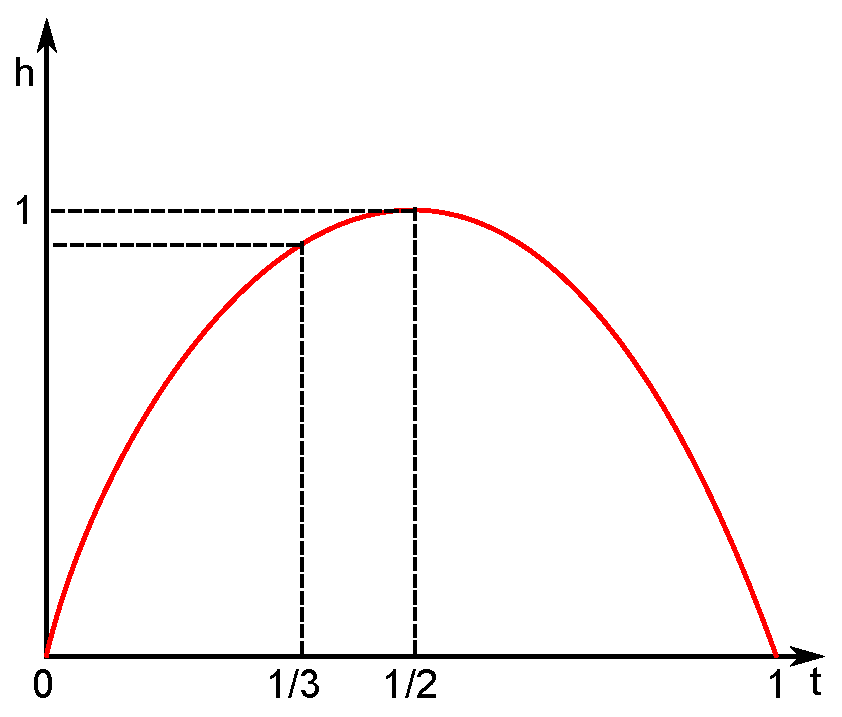
\includegraphics[width=0.6\linewidth]{pictures/ch01-i00.eps}
	\caption{The entropy function.}
\end{figure}

This function is not defined for the values $0$ and $1$. However, we have limits defined on these points and they are both $0$. So we artificially set $h(0) = 0$ and $h(1) = 0$. It is better to think about it as probability distribution $(t, 1 - t)$ and entropy is a number attached to it. Entropy measures symmetry and with $t = \ifrac{1}{2}$ we have maximum chaos (the future outcomes are equally likely).

\subsection{Lower and upper bounds}

\begin{thm}
	The upper bound on the volume of a Hamming ball, if $ r \leq \ifrac{n}{2}$, is
	$$|\hball{0}{r}| \leq 2^{nh\left(\sfrac{r}{n}\right)}$$
\end{thm}

In order to prove this theorem an analogy is introduced. Suppose there is a box with a number of chickens in it. We want to count those animals without withdrawing all of them out of the box. What can be done is to take the lightest one and measure its weight $w$; then also the weight $W$ of the box is measured. The number of the total chickens in the box can't be greater than $\ifrac{w}{W}$.\\

\noindent\textbf{Proof.} In this proof we will use a similar technique. Consider $\{0, 1\}^n$. We ``sparkle'' a substance on the strings in the set; this substance looks like probability, but it doesn't matter. Define the weight of $1$ and $0$ as 
$$P(1) = \dfrac{r}{n},\ P(0) = 1 - P(1).$$

Notice that is not an uniform distribution. Define the weight of a string as
$$P^n(\str{x}) = \prod_{i = 1}^n P(x_i).$$

If $A \subseteq \{0, 1\}^n$ then the weight of the set $A$ is $$P^n(A) = \sum_{\str{x} \in A} P^n(\str{x}).$$

$P^n(\{0, 1\}^n)$ is the total weight of the substance sparkled on the strings and it is the probability distribution of binomial. For this reason one can claim that
$$1 = P^n(\{0, 1\}^n) \geq P^n(\hball{0}{r}) = \sum_{\str{x} \in \hball{0}{r}} P^n(\str{x})$$

at this point we ``take out the lightest chicken'' and write
$$\sum_{\str{x} \in \hball{0}{r}} P^n(\str{x}) \geq |\hball{0}{r}| \cdot \min_{\str{x} \in \hball{0}{r}}P^n(\str{x})$$

Which are the lightest chickens? Because we assume $r \leq \ifrac{n}{2}$ then
$$r \leq \dfrac{n}{2} \Rightarrow P(1) = \dfrac{r}{n} \leq \dfrac{1}{2} \Rightarrow P(1) \leq P(0).$$
It follows that the the lightest strings are the ones on the border of the ball, with $r$ $1$'s. We now compute their weight.

\[\min_{\str{x} \in \hball{0}{r}}P^n(\str{x}) = [P(1)]^r\cdot[P(0)]^{n-r} = \] 
\[ = \left(\dfrac{r}{n}\right)^r \left(1 - \dfrac{r}{n}\right)^{n-r} = \]  \[ = \left(\dfrac{r}{n}\right)^{n\sfrac{r}{n}} \left(1 - \dfrac{r}{n}\right)^{n\left(1 - \sfrac{r}{n}\right)} =\]
\[ = [\left(\dfrac{r}{n}\right)^{\sfrac{r}{n}} \left(1 - \dfrac{r}{n}\right)^{\left(1 - \sfrac{r}{n}\right)}]^n =\] 
\[ =2^{n\log_2[\left(\sfrac{r}{n}\right)^{\sfrac{r}{n}}  \left(1 - \sfrac{r}{n}\right)^{\left(1 - \sfrac{r}{n}\right)}]} = \]
\[ =2^{n[\sfrac{r}{n}\log_2\sfrac{r}{n} + \left(1 - \sfrac{r}{n}\right)\log_2\left(1 - \sfrac{r}{n}\right)]} = 2^{-nh\left(\sfrac{r}{n}\right)}\]

So we have 

\[1 \geq |\hball{0}{r}| \dfrac{1}{2^{nh(\sfrac{r}{n})}} \Rightarrow |\hball{0}{r}| \leq 2^{nh\left(\sfrac{r}{n}\right)}\] 
\hfill$\Box$


\begin{thm}
	The lower bound on the volume of a Hamming ball, if $ r \leq \ifrac{n}{2}$, is
	$$|\hball{0}{r}| \geq \dfrac{1}{n+1}2^{nh(\sfrac{r}{n})}$$
\end{thm}

\noindent\textbf{Proof.} $$P(1) = \dfrac{r}{n},\ P(0) = 1 - P(1),\ P^n(\{0, 1\}^n) = 1.$$
Consider the set of all strings of length $n$ and partition it in the following way.
$$\Tau_q^n = \{\str{x}\ |\ \hweight{x} = q\},$$
obtaining $n +1$ classes. 
We know that $|\Tau_q^n| = \binom{n}{q}$; we are not interested in how many strings are in that set, but what is the total weight; we want to prove $$ |T_r| \geq \dfrac{1}{n+1}2^{nh\left(\sfrac{r}{n}\right)}.$$ There is not symmetry in the weight of the partitions so there is a weight $r$ so that
$$ \dfrac{P^n(\Tau_q)}{P^n(\Tau_r)} \leq 1,\ \forall q$$
In the formula above there are binomials we want to bound.

\begin{obs}
	$$\dfrac{k!}{l!} \leq k^{k-l}.$$
\end{obs}

\noindent\textbf{Proof}. We are going to prove this observation in two steps.
\begin{itemize}
	\item $k \geq l$. 
	$$\dfrac{k!}{l!} = \dfrac{k(k-1) \cdots l(l -1) \cdots 1}{l(l -1) \cdots 1} \leq k^{k-l}.$$
	
	\item $k < l$.
	$$\dfrac{k!}{l!} = \dfrac{k(k-1) \cdots 1}{l(l -1) \cdots k(k-1) \cdots 1} \leq \left(\dfrac{1}{k+1}\right)^{l-k} < \left(\dfrac{1}{k}\right)^{l-k} = k^{k-l}.$$
\end{itemize}
\hfill$\Box$

% Lesson5
Define $p = \ifrac{r}{n}$  so that we have a distribution $P(p, 1-p)$ that picks a set and concentrate the weight (probability) on it. We observe that the probability of each string in a class depends only on the number of $1$'s in it. So we can write

\[\dfrac{P^n(\Tau_q)}{P^n(\Tau_r)} = \dfrac{p^q(1-p)^{n-q}|\Tau_q|}{p^r(1-p)^{n-r}|\Tau_q|} = p^{q-r}(1-p)^{r-q} \dfrac{\frac{n!}{q!(n-q)!}}{\frac{n!}{r!(n-r)!}} = \]
\[ = p^{q-r}(1-p)^{r-q}\dfrac{r!}{q!}\dfrac{(n-r)!}{(n-q)!} \leq p^{q-r}(1-p)^{r-q}r^{r-q}(n-r)^{q-r} = \]

considering that $r = np$ it follows that

\[p^{q-r}(1-p)^{r-q} (np)^{r-q}[n(1-p)]^{q-r}= \] \[ = p^{q-r}(1-p)^{r-q}n^{r-q+q-r}p^{r-q}(1-p)^{q-r} = \]

\[ = p^{q-r + r-q}(1-p)^{r-q+q-r} = 1.\]

So we can write

\[1 = P^n(\{0,1\}^n) = P^n\left(\bigcup_{q=0}^nT_q\right) = \sum_{q=0}^nP^n(T_q)\leq(n+1) \max_qP^n(T_q) = \]

\[=(n+1)P^n(T_r) = (n + 1)|T_r|2^{-nh\sfrac{r}{n}}\]

From the previous result we know $|T_r| \geq \dfrac{1}{n+1}2^{nh(\sfrac{r}{n})}$ and $T_r \subseteq \hball{0}{r}$ so it follows that $|T_r| \leq |\hball{0}{r}|$. \hfill $\Box$

So this proof is important because the cardinality of the Hamming ball comes up in many contexts, such as error correction (a string that has been haltered at most $r$ times is in a certain radius from the original string).

\section{Generalization to any finite alphabet}

Let $\xset$ be the (usual) finite set that is an alphabet. The interest lies in sequences of elements of $\xset$, called \emph{strings} or \emph{words}. So $\xset^n, n \in \mathbb{N}$, is a set of words. $\xset^n$ can be partitioned by putting together those sequences that can be transformed one into the other by permutation, i. e. sequences that have the same number of occurrences of elements in the alphabet.

Let $a \in \xset$ and $\str{x} \in \xset^n$. We define the frequency of an alphabet symbol $a$ in a string $\str{x}$ in the following way:  
\begin{equation}
N(a | \str{x}) = |\{i\ |\ x_i = a\}|,
\end{equation}

where $\str{x} = x_1x_2\ldots x_n$. One can think about ``normalized'' relative frequencies of symbols $$\dfrac{1}{n} N(a|\str{x}).$$

Moreover the following holds:

$$\sum_{a \in \xset} N(a|\str{x}) = n \Rightarrow \sum_{a\in \xset} \dfrac{1}{n}N(a|\str{x}) = 1$$

so from a string $\str{x}$ one can obtain a probability distribution over $\xset$. We define
\begin{equation}
	P_{\str{x}} = \left\{ \dfrac{N(a|\str{x})}{n}\ |\ a \in \xset \right\}
\end{equation}
to be the \emph{type} of $\str{x}$. There are just that many distributions for a number $n$; now fix a distribution $P|\xset$. $\exists \str{x} \in \xset^n$ such that  $P_{\str{x}} = P$? Yes, if and only if
$$P(a) = \dfrac{N(a | \str{x})}{n},\ \forall a \in \xset.$$ Consider a product measure over $\xset$; strings in the same partition have also the same ``length'' or measure. Now, given $\xset$ and $n$, how many distributions $P|\xset$ are types in $\xset^n$? A rough upper bound is $(n + 1)^{|\xset|}$. The last value is redundant, since the values sum up to $1$. So we could do better with $(n + 1)^{|\xset| - 1}.$ We can partition $\xset^n$ into sets of strings of the same type, $\Tau_p$, with $P|\xset$. $$\Tau_p = \Tau_p^n = \{\str{x}\ |\ P_{\str{x}} = P\}.$$

\begin{thm} \label{thms:taupcard}
	If $\Tau_p \not= \emptyset$ then $$\dfrac{1}{(n+1)^{|\xset| -1}}2^{nH(p)}\leq |\Tau_p| \leq 2^{nH(p)}$$
\end{thm}

\noindent\textbf{Proof.} In order to prove the above theorem, we first define the product distribution $P|\xset \rightarrow P^n|\xset^n$ as 
\begin{equation}
	P^n(\str{x}) = \prod_{i = 1}^nP(x_i).
\end{equation}

We can define it additively on subsets of $\xset^n$.
\[
1 = P^n(\xset^n) \geq P^n(\Tau_p^n)
\]

We also introduce the \emph{generalized entropy} $H(P)$, defined as $$H(P) = -\sum_{a \in \xset} P(a)\log_2P(a).$$
Now,

\[
\forall \str{x} \in \Tau_p^n P^n(\str{x}) = \prod_{a \in \xset}P(a)^n = nP(a)
\]
notice that this is independent from $\xset$. So we have

\[ 
= \prod_{a \in \xset} 2^{nP(a)\log_2P(a)} = 2^{n\left[\sum_{a \in \xset} P(a)\log_2P(a)\right]} = 2^{-nH(p)}
\]

So,

\[1 = P^n(\xset^n) \geq P^n(\Tau^n_p) = |\Tau_p^n|2^{-nH(p)} \] $\hfill\Box$

The lower bound proof is a straightforward generalization of what has been don in the binary case. Entropy is greatest when the distribution is uniform. Now, to prove the lower bound, consider
\[
1 = \sum_{P\ |\ \Tau_p^n \not= \emptyset}P^n(\Tau_p^n) \leq (n+1)^{|\xset|-1} \max_{Q|\xset}P^n(\Tau_q^n).
\]

\begin{obs}
If $\Tau_p \not= \emptyset$ then $$\dfrac{P^n(\Tau^n_q)}{P^n(\Tau^n_p)} \leq 1$$
\end{obs}

If a distribution is a type, it maximizes its (product) value on the strings of that type. We can suppose without loss of generality (w.l.o.g) that $\Tau^n_q \not= \emptyset$.
\[
P^n(\Tau_q^n) = \prod_{a \in \xset} P(a)^{nQ(a)}|\Tau_q^n| \Rightarrow \dfrac{P^n(\Tau_q^n)}{P^n(\Tau_p^n)} = \dfrac{|\Tau_q|^n\prod_{a \in \xset}[P(a)]^{nQ(a)}}{|\Tau_p|^n\prod_{a \in \xset}[P(a)]^{nP(a)}} =
\]

\[
 = \dfrac{\dfrac{n!}{\prod_{a\in\xset}[nQ(a)]!}\prod_{a\in\xset}[P(a)]^{nQ(a)}}
 {\dfrac{n!}{\prod_{a\in\xset}[nP(a)]!}\prod_{a\in\xset}[P(a)]^{nP(a)}} = \prod_{a \in\xset} \dfrac{[nP(a)]!}{[nQ(a)]!}\prod_{a\in\xset}[P(a)]^{n(Q(a)-P(a))}\leq 
\]

\[
\leq \prod_{a \in \xset} [nP(a)]^{n(P(a)-Q(a)}\prod_{a\in\xset}[P(a)]^{n(Q(a)-P(a))} =
\]
\[
 = n^{n\left[\sum_{a \in \xset}P(a) - Q(a)\right ]} \dfrac{\prod_{a \in \xset}[P(a)]^{n(P(a)-Q(a)}}{\prod_{a \in \xset}[P(a)]^{n(P(a)-Q(a)}} =
\]

\[ 
= n^{n\left [\sum_{a \in\xset}P(a) -\sum_{a \in\xset}Q(a) \right]} = n^{n[1-1]} = 1.
\]


	\chapter{The log sum inequality}

We now prove a consequence of the concavity of the logarithm, which will be used to prove some results about entropy.

\begin{obs}[Logarithm cap-convex] \label{obs:cap-convex}
	The logarithm function is cap-convex ($\cap$-convex).
	Remember that $\ln(t) \le t - 1$ (with equality if and only if $t=1$) and $\log_2(t) = \frac{\ln(t)}{\ln(2)}$.
\end{obs}

\begin{prop}[Log sum inequality]\label{prop:logsum}
	Let $a_i \ge 0$, for $i \in \{1, 2, \dots, t\}$, $a = \sum_{i = 1}^t a_i$, and let $b_i \ge 0$, $b = \sum_{i = 1}^t b_i$, then 
	\begin{equation*}
		\sum_{i = 1}^t a_i \ln \left( \frac{a_i}{b_i} \right)
		\ge
		a \ln \left( \frac{a}{b} \right).
	\end{equation*}
\end{prop}

We are ignoring for now the cases where $a_i$ or $b_i = 0$.
The relation is with equality if and only if the two sets are proportionate, \ie $\exists c : a_i = c \cdot b_i$, $\forall i$.
When $a = b = 1$ we have two distributions $P|[t]$ and $Q|[t]$.
So:
\begin{equation*}
	\sum_{i = 1}^t P(i) \ln \left( \frac{P(i)}{Q(i)} \right) \ge 0
\end{equation*}
and we have equality if and only if $P = Q$.
We denote this with $D(P||Q)$, called the informational divergence of $P$ from $Q$.
This is not a metric (it lacks of symmetry and triangle inequality), but it can be seen as a ``dissimilarity'' measure.
It's called also Kullback-Leibler divergence or \emph{relative entropy} (From the book Elements of Information Theory, Wiley). 
 
 \Cref{prop:logsum} is based on \cref{obs:cap-convex}.
 The Proposition will be proved for the natural logarithm.
 
\begin{proof}
	We would like to prove that
	\begin{equation*}
		\sum_{i= 1}^t a_i \ln \left( \frac{a_i}{b_i} \right)
		\ge
		a \ln \left( \frac{a}{b} \right).
	\end{equation*}
	First, there is the need to set some conventions.
	When $b_i = 0$ and $a_i = 0$, we say, by convention, that
	\begin{equation*}
		0 \ln \left( \frac{0}{0} \right) = 0.
	\end{equation*}
	 
	The reason why?
	$[t] \subset [w]$, you can think of $\{a_i\}$ as a subset of some other set where the other values are all $0$s.
	Otherwise, if $a_i > 0$ and $b_i = 0$, we convene that
	\begin{equation*}
		a_i \ln \left( \frac{a_i}{b_i} \right) = +\infty.
	\end{equation*}
	We accept this convention since $b_i \geq 0$, so we can think of $\frac{a_i}{0}$ as the limit of $\frac{a_i}{f_n}$, for some $f_n \ge 0$ such that $f_n \to 0$.
	The third case is
	\begin{equation*}
	  \sum_{i = 1}^{\hat{t}} a_i \ln \left( \frac{a_i}{b_i} \right)
	  +
	  \sum_{i = \hat{t} + 1}^{t} 0 \ln \left( \frac{0}{b_i} \right)
	\end{equation*}
	with $\hat{t} < t$.
	Here we convene that
	\begin{equation*}
		0 \ln \left( \frac{0}{b_i} \right) = 0.
	\end{equation*}
	Notice that 
	\begin{equation*}
		\sum_{i = 1}^{\hat{t}} a_i \ln \left( \frac{a_i}{b_i} \right)
		+
		\sum_{i = \hat{t} + 1}^{t} 0 \ln \left( \frac{0}{b_i} \right)
		\ge a \ln \left( \frac{a}{\hat{b}} \right) + 0
		\ge a \ln \left( \frac{a}{b} \right),
	\end{equation*}
	with $\hat{b} < b$.

	Now the proof.
	First, suppose $a=b$.
	Keep in mind that
	\begin{equation*}
		\ln(x) \le x - 1
		\implies
		\ln \left( \frac{1}{x} \right) \le \frac{1}{x} - 1.
	\end{equation*}
	So,
	\begin{align*}
		\sum_{i = 1}^{t} a_i \ln \left( \frac{a_i}{b_i} \right)
		& \ge
		\sum_{i = 1}^{t} a_i \left( 1 - \frac{b_i}{a_i} \right)
		\tag{w. eq. iff $a=b$}
		\\
		& =
		\sum_{i = 1}^{t} a_i - \sum_{i = 1}^{t} a_i \frac{b_i}{a_i}
		=
		a - b = 0.
	\end{align*}
	The case then they are different can be easily reduced to this one.

	Assume $b = c \cdot a$, for $c \neq 1$.
	We introduce
	\begin{equation*}
		b_i = c \cdot \hat{b}_i \implies \hat{b}_i = \frac{b_i}{c}.
	\end{equation*}
	Then,
	\begin{align*}
		\sum_{i = 1}^{t} a_i \ln \left( \frac{a_i}{c \cdot \hat{b}_i} \right)
		& =
		\sum_{i = 1}^{t} a_i \ln \left( \frac{1}{c} \right) + \sum_{i = 1}^{t} a_i \ln \left( \frac{a_i}{\hat{b}_i} \right)
		\\
		& \ge
		\sum_{i = 1}^{t} a_i \ln \left( \frac{1}{c} \right) + a \ln \left( \frac{a}{a} \right)
		\tag{w. eq. iff $a_i = \hat{b}_i,\ \forall i$}
		\\
		& =
		a \ln \left( \frac{1}{c} \right) + a \ln \left( \frac{a}{a} \right)
		\\
		& =
		a \ln \left( \frac{a}{c \cdot a} \right)
		=
		a \ln \left( \frac{a}{b} \right). \qedhere
	\end{align*}
\end{proof}

	\chapter{Variable-length codes}

A variable-length binary code is a function 
\[
f:\msgset \rightarrow \{0, 1\}^*,\ |\msgset| < \infty,\ \{0, 1\}^* = \bigcup_{i = 1}^\infty \{0, 1\}^i.
\]
that can be extended by concatenation. If $m \in M^* \Rightarrow \exists i\ m \in M^i$. We can write $$m = m_1m_2\ldots m_i.$$ It follows that $f$ must be invertible, even after concatenation. However, the function $f^*:\msgset^* \rightarrow \{0, 1\}^*$, the extension by concatenation, defined as $$f^*(m_1\ldots m_i) = f(m_1)\ldots f(m_i),$$ is not invertible. What is needed is the prefix-free property for $f^*$.

Let $\str{x}, \str{y} \in \{0, 1\}^*$. We say that $\str{x}$ is prefix of $\str{y}$ if $\str{x} = \str{y}$ or $\exists \str{z} \in \{0, 1\}^*$ such that $\str{x}\str{z} = \str{y}$.

 So, $f$ is prefix-free if $$m'\not=m'' \Rightarrow f(m') \not\pref f(m''),$$ where ``$\pref$'' is the ``is prefix of'' relation. If $f$ is prefix-free, $f^*$ is invertible. $|f(m)| = l \Leftrightarrow f(m) \in \{0, 1\}^l$. This proposition tells us that lots of short codewords imply that the set of messages is small.

\begin{prop}[Kraft's inequality]\label{prop:kraft}
	If $f:\msgset \rightarrow \{0, 1\}^*$ is a prefix code, then $$\sum_{m\in\msgset}2^{-|f(m)|}\leq 1.$$
\end{prop}

\noindent\textbf{Proof}. Let $\str{x}, \str{v} \in \{0, 1\}^*$. Define $Y$ to be the set of all extension strings of $\str{x}$ of length $L$
$$Y_L(\str{x}) = \{\str{y}\ |\ \str{y} \in \{0, 1\}^L \wedge \str{x} \pref \str{y} \}.$$
Notice that $L < |\str{x}| \Rightarrow Y_L = \emptyset.$ Now, either $Y_L(\str{x}) \cap Y_L(\str{v}) \not= \emptyset$, or $Y_L(\str{x}) \cap Y_L(\str{v}) = \emptyset$, and maybe $Y_L(\str{x}) \subset Y_L(\str{v})$ or the other way. 
$$\str{x} \pref \str{v} \Rightarrow Y_L(\str{x}) \supseteq Y_L(\str{v}).$$
$$\str{x} \not\pref \str{v} \wedge \str{v} \not\pref \str{x} \Rightarrow Y_L(\str{x}) \cap Y_L(\str{v}) = \emptyset.$$

We say that $\prol{\str{x}}$ and $\prol{\str{v}}$ can never be in \emph{general position}. Let $A$ and  $B$ be two sets. They are in general position if $$A\cap B,\ A \setminus B,\ B \setminus A,\ \overline{A\cup B}$$ are all non-empty. For a prefix code, given $m'\not= m''$, then $$\prol{f(m')} \cap \prol{f(m'')} = \emptyset.$$ So consider $$\{0, 1\}^L \supseteq \bigcup_{m \in\msgset}\prol{f(m)},$$ and since $|\{0, 1\}^L| = 2^L$ and $$|\{0, 1\}^L| \geq \left|\bigcup_{m\in\msgset}\prol{f(m)}\right| = \sum_{m\in\msgset} |\prol{f(m)}| = \sum_{m \in \msgset} 2^{L - |f(m)|}.$$ Of course, $L \geq \max_{m \in \msgset} |f(m)|$. Now, we have
$$2^L \geq \sum_{m\in\msgset}2^{L - |f(m)|} \Rightarrow 1 \geq \sum_{m\in\msgset} 2^{-|f(m)|}.$$
$\hfill\Box$

\begin{prop}
	If $f$ is a prefix code then, for any distribution $P|\msgset$, $$\sum_{m\in\msgset}|f(m)|P(m) \geq H(P).$$
\end{prop}

\noindent\textbf{Proof}.
\[
\sum_{m \in\msgset}P(m) \log_2\left(\dfrac{P(m)}{2^{-|f(m)|}}\right) \geq 0
\]
with equality iff $P(m) = 2^{-|f(m)|}$.
\[
\sum_{m\in\msgset}P(m)\log_2(P(m)) - \sum_{m\in\msgset}P(m)\log_2(2^{-|f(m)|}) =
\]
\[
= -H(P) + \sum_{m\in\msgset}P(m)|f(m)| \geq 0 \Rightarrow H(P) \leq \sum_{m\in\msgset}P(m)|f(m)|.
\]
We have equality when $P(m) = 2^{-|f(m)|}.\hfill\Box$

\begin{obs}
	Given $P|\msgset$ it is true that $H(P) < \log(|\msgset|)$, with equality iff $P$ is the equidistribution.
\end{obs}

\noindent\textbf{Proof}.
\[
\sum_{m\in\msgset}P(m)\log\left(\dfrac{P(m)}{\sfrac{1}{|\msgset|}} \right) \geq 0
\]
with equality iff $P(m) = \ifrac{1}{|\msgset|}$
\[
\sum_{m\in\msgset}P(m)\log\left(\dfrac{P(m)}{\sfrac{1}{|\msgset|}} \right) = -H(P)+\log(|\msgset|).
\]
$\hfill\Box$

\begin{thm}[Kraft]
	Suppose $l:\msgset \rightarrow \mathbb{N}$, a prescribed codeword length, satisfies Kraft's inequality (Proposition \ref{prop:kraft}). Then 
	$\exists f:\msgset \rightarrow \{0, 1\}^*$ prefix code such that $|f(m)| = l(m),\ \forall m$.
\end{thm}

\noindent\textbf{Proof}. We prove this with a greedy algorithm. We'll find an ordering of $\msgset$, which helps us with being greedy. We order $\msgset$ so that $l(m_1) \leq l(m_2) \leq \ldots \leq l(m_{|\msgset|})$.

\noindent\textbf{First step.} Set $L = l(m_{|\msgset|}) = \max_ml(m)$. We work with strings of length $L$ and then we shorten them. Choose arbitrary $\hat{\str{x}}^{(1)} \in \{0, 1\}^L$ and let $f(m_1)$ be the prefix of $\hat{\str{x}}^{(1)}$ of length $l(m_1)$. We then exclude the set of $2^{L - l(m_1)}$ extensions of $f(m_1)$.

\noindent\textbf{General step.} After constructing strings $\str{x}_1,\str{x}_2, \ldots, \str{x}_{t-1}$, choose $\hat{\str{x}}^{(t)}$ from $\{0, 1\}^L \setminus (\prol{\str{x}_1} \cup \cdots \cup \prol{\str{x}_{t-1}})$. Then $\str{x}_t = $ the prefix of length $l(m_t)$ of $\hat{\str{x}}^{(t)}$.

We have to prove that the algorithm ends giving to each string in $\msgset$ an image, and that it builds a prefix code.

\noindent Suppose that the algorithm stops at step $t$. Then $\{0, 1\}^L = \bigcup_{i = 1}^{t-1}\prol{\str{x}_i}$. We have seen that $|\prol{\str{x}_i}| = 2^{L - l(m_i)}$. This means that

\[
2^L = \left|\bigcup_{i=1}^{t-1}\prol{\str{x}_i} \right| \leq \sum_{i=1}^{t-1}|\prol{\str{x}_i}| = \sum_{i=1}^{t-1} 2^{L-l(m_i)}
\]
dividing by $2^L$ we obtain
$$1 \leq \sum_{i=1}^{t-1}2^{-l(m_i)}$$
in contradiction with Kraft's inequality (Proposition \ref{prop:kraft}), since we have at least $t$ messages. 

%If $t < |\msgset|$ then $$\sum_{i=1}^{t} 2^{L-l(m_i)} < 2^L$$ so the procedure terminates.

\noindent\emph{Correctness}. $f$ is a prefix-code. We have to show that $$i \not= j \Rightarrow \prol{\str{x}_i} \cap \prol{\str{x}_j} = \emptyset.$$
Since they are not in general position, we just have to show that they don't contain one another. $$\prol{\str{x}_t} \not\supset \prol{\str{x}_i},\ i < t,$$ since $l(m_i) \leq l(m_t)$, $|\prol{\str{x}_i}| \geq |\prol{\str{x}_t}|$. The sets get smaller and smaller. On the other hand

$$\prol{\str{x}_t} \not\subset \prol{\str{x}_i},\ i < t$$
recall that $\hat{\str{x}}^{(t)}$ was chosen in such a way that $\hat{\str{x}}^{(t)} \in \prol{\str{x}_t}$, and that $\hat{\str{x}}^{(t)} \not\in \prol{\str{x}_i},\ \forall i < t$. So $\prol{\str{x}_t}$ has an element not in $\prol{\str{x}_i}$, so it can't be included.

$\hfill\Box$

If our code does not satisfy Kraft's inequality to equality, \emph{i.e.} $$\sum_{m\in\msgset}2^{-|f(m)|} < 1,$$ then $\exists \lambda \geq L, \lambda \in \mathbb{N}$ t.c. $$\sum_{m\in\msgset}2^{-|f(m)|} + 2^{-\lambda} \leq 1$$ with $l(m_1) \leq \cdots \leq l(m_{|\msgset|}) \leq \lambda$ so we could add some more words to our code. A maximal prefix code is a prefix code to which you can't add more codewords (and still get a prefix-code).

\begin{prop}
 $\forall P|\msgset\ \exists f:\msgset \rightarrow \{0, 1\}^*$ prefix code such that
 \[
  \sum_{m\in \msgset} P(m)|f(m)| < H(P) + 1
 \]
\end{prop}

\noindent\textbf{Proof}. We'll give a prescription satisfying Kraft's inequality and this inequality too. 

\[
 H(P) = \sum_{m \in \msgset} P(m)\log\left(\dfrac{1}{P(m)}\right).
\]

Let
\begin{equation}\label{eq:pres-cod-len}
l(m) = \dfrac{1}{P(m)}. 
\end{equation}

Equation \ref{eq:pres-cod-len} is not always an integer and could not satisfy Kraft's inequality. We could choose

\begin{equation}
l(m) = \left\lceil\log\left(\dfrac{1}{P(m)}\right)\right\rceil.
\end{equation}


Since $\left\lceil t \right\rceil < t + 1$ we can easily see that 

\begin{align*}
\sum_{m \in M} P(m)\left\lceil\log\left(\dfrac{1}{P(m)}\right)\right\rceil & < \sum_{m \in \msgset} P(m)\log\left(\dfrac{1}{P(m)}\right) + \sum_{m \in \msgset} P(m)\\ & =  H(P) + 1. 
\end{align*}


We now check that $l$ satisfies Kraft's inequality.

\begin{align*}
\sum_{m \in \msgset} 2^{-l(m)} & = \sum_{m \in \msgset} 2^{-\left\lceil\log\left(\sfrac{1}{P(m)}\right)\right\rceil}\\ 
& \leq\tag{here we are using $\left\lceil t \right\rceil \geq t$}
 \sum_{m \in \msgset} 2^{-\log\left(\dfrac{1}{P(m)}\right)} \\ 
& = \sum_{m \in \msgset} 2^{\log(P(m))} \\
& = \sum_{m \in \msgset} P(M) = 1.
\end{align*}

$\hfill\Box$
	\chapter{Entropy of \aclp{RV}}

Let's reason on the probability of a message.
You can consider an infinite sequence of \acp{RV} $X_i$ which take values in $\M$.
We implicitly assume that $X_i$ are independent \acp{RV}.
If we group \acp{RV} before encoding we can asymptotically reach entropy.

\section{Joint Entropy, Conditional Etropy and Mutual Information}

Given a \ac{RV} $X$, the entropy of $X$ is defined as
\begin{equation*}
	\Entropy{X} = \Entropy{P_X},
\end{equation*}
where $P_X$ is the distribution of $X$.
How is entropy defined for two \acp{RV}?
If $X = Y$ then $\Entropy{X,Y} = \Entropy{X}.$

\begin{definition}[Joint Entropy]
	In general, the entropy of a pair is the entropy of the \ac{RV} derived by the pair, \ie
	\begin{equation*}
		\Entropy{X,Y} = \Entropy{(X,Y)}, 
	\end{equation*}
	since $(X, Y)$ has a probability distribution $P_{XY}$ and we can think of the pair as just a \ac{RV}.
	$\Entropy{X,Y}$ is defined a the \emph{joint entropy} of $X$ and $Y$. 
\end{definition}

\begin{prop}
	\begin{equation*}
		\Entropy{P} \le \log_2 \left( \abs{\X} \right),
	\end{equation*}
	with $P|\X$ and with equality if and only if $P$ is the equidistribution, \ie $P(x) = \frac{1}{\abs{\X}}$ for all $x \in \X.$
\end{prop}

\begin{proof}
	Call $\U$ the uniform distribution.
	$D(P||\U)\ge 0$, with equality if and only if $P = \U$.
	\begin{align*}
		D(P||\U)
		& =
		\sum_{x \in \X} P(x) \log_2 \left( \frac{P(x)}{\frac{1}{\abs{\X}}} \right)
		\\
		& =
		\sum_{x \in \X} P(x) \log_2 \left( P(x) \right)
		+
		\sum_{x \in \X} P(x) \log_2 \left( \abs{\X} \right)
		\\
		& =
		-\Entropy{P} + \log_2 \left( \abs{\X} \right).
	\end{align*}
	This quantity is nonnegative with equality to zero if and only if $P = \U$.
\end{proof}

We write $X \in \X$ since $X$ is like an unknown element of $\X$.
Random variables don't always have an expected value.
We can think of $\Entropy{X}$ as the information content of $X$.
If we consider entropy as the amount of information in a \ac{RV}, then it should be that $\Entropy{X,Y} \ge X$.
We can think of entropy as  measure over a set.
\begin{align*}
	\Entropy{X} \sim \mu(A), & \, A \subseteq U
	\\
	\Entropy{X,Y} \sim \mu(A \cup B), & \, \mu(A \cup B) \geq \mu(A)
\end{align*}

\begin{prop}
	\begin{equation*}
		\Entropy{X,Y} \ge \Entropy{X}.   
	\end{equation*}
\end{prop}

\begin{proof}
	Consider the following quantities:
	\begin{equation*}
		\Entropy{X,Y}
		=
		\sum_{x \in \X} \sum_{y \in \Y} \Pr{X = x, Y = y}
		\log_2 \left( \frac{1}{\Pr{X = x, Y = y}} \right),
	\end{equation*}
	and
	\begin{align*}
		\Entropy{X}
		& =
		\sum_{x \in \X} \Pr{X = x} \log_2 \left( \frac{1}{\Pr{X=x}} \right)
		\\
		& =
		\sum_{x \in \X} \sum_{y \in \Y} \Pr{X = x, Y = y}
		\log_2 \left( \frac{1}{\Pr{X = x}} \right).
	\end{align*} 

	We take the difference between the two:
	\begin{equation*}
		\Entropy{X,Y} - \Entropy{X}
		=
		\sum_{x \in \X} \sum_{y \in \Y}
		\Pr{X = x, Y = y}
		\log_2 \left( \frac{\Pr{X = x}}{\Pr{X = x, Y = y}} \right).
	\end{equation*}

	The definition of conditional probability gives us that $\Pr{X = x, Y = y} = \Pr{X = x} \cdot \Pr{Y = y | X = x}$, and as such
	\begin{align*}
		\sum_{x \in \X} \sum_{y \in \Y} \Pr{X = x} \cdot \Pr{Y = y | X = x}
		\log_2 \left( \frac{1}{\Pr{Y = y | X = x}} \right)
		\\
		=
		\sum_{x \in \X} \Pr{X = x} \sum_{y \in \Y} \Pr{Y = y | X = x}
		\log_2 \left( \frac{1}{\Pr{Y = y | X = x}} \right).
	\end{align*}
	We would like to say that this quantity is nonnegative.
	Since $\Entropy{\cdot}$ is nonnegative, this difference is actually greater than (or equal to) zero.
\end{proof}

\begin{definition}[Conditional Entropy]
	We call
	\begin{equation*}
		\Entropy{Y | X} = \Entropy{X,Y} - \Entropy{X}
	\end{equation*}
	the \emph{conditional entropy} of $Y$ given $X$.
\end{definition}

$\Entropy{X,Y} - \Entropy{X}$ is the convex combination of the entropies of the conditional distribution of $Y$ given the various values of $X$.
It's like the expected value of the entropy of the conditional distribution $\Pr{Y = y | X = x}$.
It can be seen as the residual information when $X$ is known.

\begin{prop}
	\begin{equation*}
	\Entropy{Y} \ge \Entropy{Y | X}. 
	\end{equation*}
\end{prop}

\begin{proof}
	\begin{align*}
		\Entropy{Y} - \Entropy{Y | X}
		= &
		\sum_{x \in \X} \sum_{y \in \Y} \Pr{X = x, Y = y}
		\log_2 \left( \frac{1}{\Pr{Y=y}} \right)
		\\ 
		&~- \sum_{x \in \X} \sum_{y \in \Y} \Pr{X = x, Y = y}
		\log_2 \left( \frac{\Pr{X = x}}{\Pr{X = x, Y = y}} \right)
		\\
		= &
		\sum_{x \in \X} \sum_{y \in \Y} \Pr{X = x, Y = y}
		\log_2 \left( \frac{\Pr{X = x, Y = y}}{\Pr{X = x} \cdot \Pr{Y = y}} \right).
	\end{align*}
	This is symmetrical in $X$ and $Y$.
	Notice that $\Entropy{Y} - \Entropy{Y | X}$ is not.
	This also looks as a log sum inequality.
	In Particular, it is similar to information divergence of the distribution $P_{XY}$ from the distribution $P_X \times P_Y$. So,
	\begin{equation*}
		\Entropy{Y} - \Entropy{Y | X}
		=
		D \left( P_{XY} || P_X \times P_Y \right)
		\ge 0,
	\end{equation*}
	and we have equality when $P_{XY} = P_X \times P_Y$.
	It is a measure of indipendence of $X$ and $Y$.
\end{proof}

\begin{definition}[Mutual Information]
	We define the amount of information that $X$ and $Y$ share as follows:
	\begin{equation*}
		\MutualInformation{X \land Y} = \Entropy{Y} - \Entropy{Y | X}, 
	\end{equation*}
	and it is called mutual information.
	It is symmetric and nonnegative. 
\end{definition}

Notice that
\begin{align*}
	\MutualInformation{X \land Y}
	& =
	\Entropy{Y} - \Entropy{Y | X}
	\\
	& =
	\Entropy{Y} + \Entropy{X} - \Entropy{X,Y} 
\end{align*}
thus
\begin{equation*}
	\Entropy{X,Y} \le \Entropy{X} + \Entropy{Y} 
\end{equation*}
with equality if and only if $X$ and $Y$ are independent.
Finally, we state (without proof) that
\begin{equation*}
	\Entropy{Y | Z} \ge \Entropy{Y | Z, X}.
\end{equation*}

\begin{prop}[Chain Rule] \label{prop:chain-rule}
	The \emph{chain rule} states that
	\begin{equation*}
		\Entropy{X_1, \dots, X_n}
		=
		\Entropy{X_1}
		+
		\sum_{i = 2}^n \Entropy{X_i | X_1, \dots, X_{i-1}}.
	\end{equation*}
\end{prop}

We have said that $\MutualInformation{X \land Y} \sim \mu(A \cap B)$, and since $\Entropy{Y | X, Z} \le \Entropy{Y|Z}$ we can state that
\begin{equation*}
	\MutualInformation{X \land Y | Z}
	\sim
	\mu(A \cap B \setminus C)
\end{equation*}
that is the conditional mutual information.
We now wonder about which quantity between $\MutualInformation{X \land Y | Z}$ and $\MutualInformation{X \land Y}$ is greater.
\begin{align*}
	\MutualInformation{X \land Y} -  \MutualInformation{X \land Y | Z}
	& \sim
	\mu(A \cap B) - \mu((A \cap B) \setminus C)
	\\
	& =
	\mu((A \cap B) \setminus ((A \cap B) \setminus C))
	\\ 
	& =
	\mu(A \cap B \cap C). 
\end{align*}
This is what the analogy suggests, but we need a proof to believe that this is true.
Assume that
\begin{equation}\label{eq:mutcondinf}
	\MutualInformation{X \land Y} - \MutualInformation{X \land Y | Z} \ge 0.
\end{equation}
If $X \equiv Y \equiv Z$ then
\begin{equation*}
	\MutualInformation{X \land X} = \Entropy{X} - \Entropy{X | X} = \Entropy{X},
\end{equation*}
so \cref{eq:mutcondinf} is possible.
But we can also have it the other way around:
\begin{equation*}
	\MutualInformation{X \land Y | Z} - \MutualInformation{X \land Y} \ge 0. 
\end{equation*}
It follows that the inequality of \cref{eq:mutcondinf} does not hold always.

Suppose $X, Y, Z \in \{0, 1\}$, and also they are uniformly distributed.
Moreover, $X$ and $Y$ are independent so $\MutualInformation{X \land Y} = 0$.
We then define $Z = X \xor Y$, but then $X = Y \xor Z$ and $Y = X \xor Z$.
$X, Y, Z$ are pairwise independent, but they are not three-way independent, since every couple of them determines the third.
\begin{equation*}
	\MutualInformation{X \land Y | Z}
	=
	\Entropy{X | Z} - \Entropy{X | Y, Z}
	=
	\Entropy{X} - 0
	= 1.
\end{equation*}
Any number $m \ge 2$ of sets are disjoint if and only if they are pairwise disjoint, but \ac{RV} independence does not satisfy this property.
The analogy fails on assuming that \acp{RV} independence is similar to set disjointness.
$n$-way independence is binary, but $n$-way independence is unrelated to $m$-way independence if $n \neq m$.

\section{Information Source and Speed of Information}

An \emph{information source} is an infinite sequence $X_1, X_2, \dots, X_n, \dots$ of \acp{RV} with $X_i \in \X$, \ie they take values from the same set.
How can we measure the information content in an information source?
We denote the information source as $X^\infty$, and with $X^n = X_1, \dots, X_n$ a sequence of $n$ \acp{RV}.

The ``speed'' of information from a sequence of \acp{RV} is 
\begin{equation*}
	\frac{1}{n} \Entropy{X_1, \dots, X_n}.
\end{equation*}

The information rate of $H^\infty$, if it exists, is
\begin{equation*}
	\lim_{n \to \infty} \frac{1}{n} \Entropy{X^n}. 
\end{equation*}


Consider $\{X_i\}_{i = 1}^\infty$, an infinite sequence of independent and identically distributed \acp{RV}, and denote by $P$ the common distribution of $\{X_i\}_{i = 1}^\infty$, so that $\Entropy{X_i} = \Entropy{P}$ for all $i$.

In this case,
\begin{equation*}
	\Entropy{X_1, \dots, X_n}
	=
	\sum_{i = 1}^n \Entropy{X_i}
	=
	n \cdot \Entropy{P},
\end{equation*}
so
\begin{equation*}
	\lim_{n \to \infty} \frac{1}{n} \Entropy{X^n} = \Entropy{P}.
\end{equation*}

What is the sufficient condition for this to hold (\ie for the limit to exists)?
We need stationary \acp{RV}: impredictable but ``stationary''. 
\begin{definition}[Stationary Information Source]
	We call an information source $\{X_i\}_{i = 1}^\infty$ \emph{stationary} if 
	\begin{equation*}
		\forall n,k \in \Naturals, \forall \str{x} \in \X^n
		.
		\Pr{X^n = \str{x}} = \Pr{X_{k+1}, \dots, X_{k+n} = \str{x}}.
	\end{equation*} 
\end{definition}

We will see that if an information source is stationary then it has an information rate.
In particular, with a stationary source the entropy of a sequence
\begin{equation*}
	\Entropy{X_i | X_1, \dots, X_{i-1}}
\end{equation*}
decreases.

\begin{definition}[Memoryless Information Source]
	We call an information source \emph{memoryless} if $X_i$, for all $i$, are totally independent.  
\end{definition}
We will show that lack of memory is not a sufficient condition for the existence of the information rate.

Consider $\{X_i\}_{i = 1}^\infty$, a sequence of totally independent \acp{RV}, does its entropy rate exists?

\begin{equation*}
	\frac{1}{n} \cdot \Entropy{X_1, \dots, X_n}
	=
	\frac{1}{n} \sum_{i = 1}^n \Entropy{X_i}.
\end{equation*}
When does this quantity diverge?
Take $\Entropy{X_i} \in \{0, 1\}$, what we want to know is if it exists the following limit, for $\epsilon_i \in \{0,1\}$:
\begin{equation*}
	\lim_{n \to \infty} \sum_{i = 1}^n \frac{\epsilon_i}{n}.
\end{equation*}

Consider the following information source:
\begin{equation*}
	\overbrace{0101\dots0101}^{n \text{ bits}}
	\overbrace{0101\dots0101}^{n \text{ bits}}
	\overbrace{1111\dots1111}^{2n \text{ bits}}.
\end{equation*}
The first $2n$ bits, a sequence of alternating bits, have average $\frac{1}{2}$.
Add the second $2n$ and you get $\frac{3}{4}$.
Repeat this and the sequence oscillates between $\frac{3}{4}$ and $\frac{1}{2}$.

\begin{thm}[Information rate of a stationary source]
	If $\{X_i\}_{i = 1}^\infty$ is stationary, then its entropy rate exists.
\end{thm}

\begin{proof}
	It's reasonable to think that
	\begin{equation*}
		\frac{1}{n} \cdot \Entropy{X_1, \dots, X_n}
	\end{equation*}
	goes to 0.
	What we are going to prove is that this is in fact true, and thus the information rate of a stationary information source exists (and it is 0).

	To prove it, we just have to show that the sequence is decreasing, since $\Entropy{\cdot}$ is always positive, \ie we show that
	\begin{equation*}
		\frac{1}{n} \cdot \Entropy{X_1, \dots, X_n}
		\le
		\frac{1}{n-1} \cdot \Entropy{X_1, \dots, X_{n-1}},
	\end{equation*}
	which we could also write as
	\begin{equation*}
		(n-1) \cdot \Entropy{X^n}
		\le
		n \cdot \Entropy{X^{n-1}},
	\end{equation*}
	that is equal to saying that
	\begin{equation*}
		(n-1) \cdot \left[ \Entropy{X^{n-1}} + \Entropy{X_n | X^{n-1}} \right]
		\le
		n \cdot \Entropy{X^{n-1}}.
	\end{equation*}

	Thus,
	\begin{equation*}
		(n-1) \cdot \Entropy{X_n | X^{n-1}} \le \Entropy{X^{n-1}}
	\end{equation*}

	We apply the definition of joint entropy (\cref{prop:chain-rule}):
	\begin{equation*}
		(n-1) \cdot \Entropy{X_n | X^{n-1}}
		\le
		\Entropy{X_1} + \sum_{i=2}^{n-1} \Entropy{X_i | X^{i-1}}
	\end{equation*}

	Since the source is stationary, $\Entropy{X^{n-1}} = \Entropy{X_2, \dots, X_n}$, and we can rewrite the \ac{RHS} as follows:
	\begin{align*}
		\Entropy{X_1} + \sum_{i=2}^{n-1} \Entropy{X_i | X^{i-1}}
		& =
		\Entropy{X^{n-1}}
		=
		\Entropy{X_2, \dots, X_{n}}
		\\
		& =
		\Entropy{X_{n}, \dots, X_2}
		\\
		& =
		\Entropy{X_n} + \sum_{i=2}^{n-1} \Entropy{X_n | X_{1 + n - i}, \dots, X_{n-1}}.
	\end{align*}

	Our thesis thus becomes
	\begin{equation*}
		(n-1) \cdot \Entropy{X_n | X^{n-1}}
		\le
		\Entropy{X_n} + \sum_{i=2}^{n-1} \Entropy{X_n | X_{1+n-i}, \dots, X_{n-1}}.
	\end{equation*}
	This is a weaker statement than the following $n-1$ statements:
	\begin{align*}
		\Entropy{X_n | X^{n-1}} \le~& \Entropy{X_n},
		\\
		& \vdots
		\\
		\Entropy{X_n | X^{n-1}} \le~& \Entropy{X_n | X_{1+n-i}, \dots, X_{n-1}},
		\\
		& \vdots
		\\
		\Entropy{X_n | X^{n-1}} \le~& \Entropy{X_n | X^{n-1}}.
	\end{align*}
	We have coupled the $n-1$ terms in the \ac{LHS} with one of the $n-1$ terms in the \ac{RHS}.

	Look at the generic term: for all $k$,
	\begin{equation*}
		\Entropy{X_n | X_1, \dots, X_{n-1}}
		\le
		\Entropy{X_n | X_{n-k}, \dots, X_{n-1}}.
	\end{equation*}
	By definition of mutual information, we have that
	\begin{align*}
		\Entropy{X_n | X_{n-k}, \dots, X_{n-1}}
		-
		\Entropy{X_n | X_1, \dots, X_{n-1}}
		& =
		\\
		\MutualInformation{X_n \land X_1 \land \dots \land X_{n-k-1} | X_{n-k}, \dots, X_{n-1}}
		& \ge 0. \qedhere
	\end{align*}

	This reminds us that
	\begin{align*}
		\MutualInformation{A \land B | C} \ge 0
		\implies
		\Entropy{A | C} \ge \Entropy{A | B, C}.
	\end{align*}
\end{proof}

\section{Universal Compression}

Lempel and Ziv worked on universal compression algorithms.
Universal compression is possible with stationary source.
How would you compress a stationary source to its entropy?

Consider a stationary information source $\{X_i\}_{i=1}^\infty$.
Given $f$, a variable length prefix code, we consider $\abs{f(X_i)}$ as a \ac{RV}.
We can talk about the expected value $\expectation{\abs{f(X_i)}}$ of this \ac{RV}.
Since $\expectation{\abs{f(X_i)}} = \sum_{x \in \X} \Pr{X_i = x} \abs{f(x)}$, by \cref{prop:prefix-entropy-upper} and \cref{prop:prefix-entropy-lower} we know that
\begin{equation} \label{eq:universal-compression-expectation}
	\Entropy{X_i} \le \expectation{\abs{f(X_i)}} \le \Entropy{X_i} + 1.
\end{equation}
Note that the length of the string obtained by applying $f$ to $n$ \acp{RV} is
\begin{equation*}
	\abs{f(X_1), \dots, f(X_n)} = \sum_{i=1}^n \abs{f(X_i)},
\end{equation*}
and that, by \cref{eq:universal-compression-expectation} above,
\begin{equation*}
	\frac{1}{n} \sum_{i=1}^n \Entropy{X_i}
	\le
	\frac{1}{n} \sum_{i=1}^n \abs{f(X_i)}.
\end{equation*}

If the source is stationary all \acp{RV} have the same probability distribution $P$, and thus
\begin{equation*}
	\Entropy{P} \le \frac{1}{n} \sum_{i = 1}^n \abs{f(X_i)} \le \Entropy{P} + 1,
\end{equation*}
but this does not tell us much.

Instead, we join \acp{RV} together.
Let $f_n$ be an optimal (in the sense of length of output) prefix code for $X_1, \dots, X_n$.
\begin{equation*}
	\frac{1}{k} \cdot \Entropy{X^k}
	\le
	\frac{1}{k} \cdot \expectation{\abs{f_n \left( X^k \right)}}
	\le
	\frac{1}{k} \cdot \left[ \Entropy{X^k} + 1 \right].
\end{equation*}
If $k \to \infty$ (and we enlarge the conding window), both sides go to the entropy rate.
Thus the entropy is the ``limit''.

	
\chapter{\aclp{ECC}}

\acp{ECC} arise in probabilistic contexts.
Consider a memory device with $n$ cells.
We can model the content as a string $\str{x} \in \{0, 1\}^n$.
The device decays; each cell can flip its value independently from the others with a certain probability (uniform).
The probability $p$ is usually $< 1/2$.
We can expect no more than $np$ flips.
Can we guarantee recovery from so many errors?
Yes, thanks to algebra.
The string $\str{x}$ can be converted into anything inside a ball of radius $np$.
We want that two strings $\str{x}$ and $\str{y}$ are distant, so that their balls do not intersect.
The pairwise distance of the words should be $\ge 2np + 1$.

Let $\C \subseteq \{0, 1\}^n$ be a codeblock.
The first property that we want from $\C$ is that $\abs{\C}$ should be large.

Next, we extend the definition of Hamming Distance to sets, \ie we define
\begin{equation*}
	\hdist{\C} = \min_{\{\str{x}, \str{y}\} \in \binom{\C}{2}} \hdist{\str{x}, \str{y}},
\end{equation*}
where 
\begin{equation*}
	\binom{\C}{2} = \left\{ \{\str{x}, \str{y}\}\ |\ \str{x}, \str{y} \in \C \land \str{x} \neq \str{y} \right\}. 
\end{equation*}
So $\hdist{\C}$ tells how close the closest elements of $\C$ are.
$\hdist{\C}$ should be large too.

What is the best possible trade-off?
\begin{equation*}
	M(n, d) = \max_{\C \subseteq \{0,1\}^{n} : \hdist{\C} \ge d} \abs{\C}
\end{equation*}
This says that we are concentrating on codes for which $\hdist{\C} \ge d$ for some $d$.

We can think of the graph for which $V = \{0, 1\}^n$ and $\str{x}, \str{y} \in \binom{V}{2}$ share an edge if and only if $\hdist{\str{x}, \str{y}} \ge d$.
$M(n,d)$ is the size of the largest clique in this graph.

We try to make this simpler by looking at the problem from an asymptotic point of view.
We consider $M(n, n \delta)$ for $\delta \in [0, 1]$.
This grows to infinity exponentially in $n$, while
\begin{equation*}
	\frac{1}{n} \log_2 \left( M(n, n \delta) \right)
\end{equation*}
does not grow exponentially.
So we look at the superior limit of
\begin{equation*}
	R(\delta) = \limsup_{n \to \infty} \frac{1}{n} \log_2 \left( M(n, n \delta) \right).
\end{equation*}
$R$ here stands for \emph{rate}.

$M(n, n \delta)$ is the size of largest set of strings one can put inside $n$ bits of memory, with minimum distance $n \delta$.
Its logarithm is the number of bits of true information that we can store.
Dividing by $n$ we get the amount of information bit by bit.
We can easily see that $R(0) = 1$ and that $R(1) = 0$.

\begin{thm}[Gilbert-Varshamov bound] \label{thm:gilbert-varshamov}
	If $\delta \in \left[ 0, \frac{1}{2} \right]$, then
	\begin{equation*}
		R(\delta) \ge 1 - \entropy{\delta}.
	\end{equation*}
\end{thm}

\begin{proof}
	This means that
	\begin{equation*}
		M(n, n \delta) \ge 2^{n \, \left[1 - \entropy{\delta} \right]}.
	\end{equation*}
	This bound was later improved to $n 2^{n \, \left[1 - \entropy{\delta} \right]}$.

	For now, fix $n, d \in \Naturals$.
	Take an arbitrary string $\str{x} \in \{0, 1\}^n$, and exclude $\hball{\str{x}}{d-1}$ from our future choices.

	Then, after having found $\str{x}_1, \dots, \str{x}_{t-1}$, we choose arbitrarily
	\begin{equation*}
		\str{x}_t \in \{0, 1\}^n \setminus \bigcup_{i = 1}^{t-1} \hball{\str{x}_i}{d-1},
	\end{equation*}
	so, after picking each string, we exclude the Hamming Ball of radius $d-1$ around it from our future choices.

	How long can this go on?
	Maybe after $m$ steps we have that
	\begin{equation*}
		\{0, 1\}^n \setminus \bigcup_{i = 1}^{m} \hball{\str{x}_i}{d-1} = \emptyset.
	\end{equation*}

	How large $m$ can be?
	We stop when 
	\begin{align*}
		\{0, 1\}^n
		& \subseteq
		\bigcup_{i = 1}^{m} \hball{\str{x}_i}{d-1}
		\\
		& \implies
		\\
		2^n
		& \le
		\abs{\bigcup_{i = 1}^{m} \hball{\str{x}_i}{d-1}}
		\\
		& \le
		\sum_{i = 1}^m \abs{\hball{\str{x}_i}{d-1}}
		\\
		& \le
		\sum_{i = 1}^m \abs{\hball{\str{x}_i}{d}}
		\\
		& \le
		m 2^{n \, \entropy{\frac{d}{n}}},
	\end{align*}
	where the last inequality holds since $d \le \frac{n}{2}$.
	We have proven the thesis, since now
	\begin{equation*}
		M(n, d) \ge m \ge \frac{2^n}{2^{n \, \entropy{\frac{d}{n}}}}
		=
		2^{n \, \left[ 1 - \entropy{\frac{d}{n}} \right]},
	\end{equation*}
	where $\frac{d}{n} = \delta.$
\end{proof}

\begin{thm}[Hamming bound] \label{thm:hamming-bound}
	For $\delta \in [0, 1]$,
	\begin{equation*}
		R(\delta) \le 1 - \entropy{\frac{\delta}{2}}.
	\end{equation*}
\end{thm}

\begin{proof}
	Fix $n, d \in \Naturals$, $\hdist{\C} \ge d$, arbitrarily.

	Consider the centres $\str{x}$ and $\str{y}$ of two Hamming balls, with $\hdist{\str{x}, \str{y}} = d$.
	For the two Hamming balls to be disjoint, we must choose
	\begin{equation*}
		\hball{\str{x}}{\frac{d-1}{2}}
		\text{ and }
		\hball{\str{y}}{\frac{d-1}{2}}.
	\end{equation*}

	Assume the two Hamming Balls are not disjoint, \ie
	\begin{equation*}
		\hball{\str{x}}{\frac{d-1}{2}}
		\cap
		\hball{\str{y}}{\frac{d-1}{2}}
		\neq \emptyset;
	\end{equation*}
	but this means that
	\begin{equation*}
		\exists \str{z} \in
		\hball{\str{x}}{\frac{d-1}{2}}
		\cap
		\hball{\str{y}}{\frac{d-1}{2}},
	\end{equation*}
	and that, since $\str{z}$ is in both Hamming Balls,
	\begin{equation*}
		\hdist{\str{x},\str{z}} \le \frac{d-1}{2}
		\qquad
		\hdist{\str{y},\str{z}} \le \frac{d-1}{2}.
	\end{equation*}
	But then we have that
	\begin{equation*}
		d = \hdist{\str{x},\str{y}}
		\le
		\hdist{\str{x},\str{z}} + \hdist{\str{y},\str{z}}
		\le
		2 \cdot \frac{d-1}{2}
		= d-1 < d,
	\end{equation*}
	in contradiction with the assumption that $\hdist{\str{x},\str{y}} = d$.

	If all strings have a distance of at least $d$, we can correct up to $\frac{d-1}{2}$ errors.

	Assume $\C$ is built using disjoint balls, and that $M(n, d) = \abs{\C}$.
	Then
	\begin{equation*}
		\abs{\bigcup_{\str{x} \in \C} \hball{\str{x}}{\frac{d-1}{2}}}
		=
		\abs{\C} \cdot \abs{\hball{\zero}{\frac{d-1}{2}}}
		\ge
		\frac{\abs{\C}}{n+1} \cdot 2^{n \, \entropy{\frac{d-1}{2n}}}.
	\end{equation*}
	Now, since the Hamming Balls are disjoint, we have that
	\begin{equation*}
		\abs{\bigcup_{\str{x} \in \C} \hball{\str{x}}{\frac{d-1}{2}}} \le 2^n,
	\end{equation*}
	which in turn gives us that $M(n,d) = \abs{\C}$ can be upper bounded as
	\begin{equation*}
		M(n, d) = \abs{\C} \le (n+1) \cdot 2^{n \, \left[1 - \entropy{\frac{d-1}{2n}}\right]}.
	\end{equation*}
	
	We now take the logarithm and normalise by $n$, and obtain
	\begin{equation*}
		\frac{1}{n} \log_2 \left( M(n, d) \right)
		\le
		\frac{1}{n} \log_2 \left( n+1 \right) + 1 - \entropy{\frac{d-1}{2n}},
	\end{equation*}
	and, by taking the limit superior of that quantity, we get
	\begin{align*}
		R(\delta)
		& =
		\limsup_{n \to \infty} \frac{1}{n} \logtwo{M(n, n \delta)}
		\\
		& =
		\limsup_{n \to \infty}
		\cancelto{0}{
			\frac{1}{n} \logtwo{n+1}
		}
		+ 1 - \entropy{
			\frac{\cancel{n} \, \delta}{2 \, \cancel{n}}
			- \cancelto{0}{\frac{1}{2n}}
		},
		\\
		& \le
		1 - \entropy{\frac{\delta}{2}}. \qedhere
	\end{align*}
\end{proof}

\section{\acl{UD} codes}

\begin{definition}[\acl{UD} code]
	Let $f : \M \to \{0,1\}^{\star}$, and define $f^{\star} : \M^{\star} \to \{0,1\}^{\star}$ as
	\begin{equation*}
		f^{\star} (\str{m}) = f(m_1) f(m_2) \dots f(m_t),
	\end{equation*}
	for $\str{m} \in \M^{\star}$ with $\str{m} = m_1 m_2 \dots m_t$ for some $t$.
	We say that $f$ is \ac{UD} if $f^{\star}$ is injective.
\end{definition}
If $f$ is a prefix code, $f$ is \ac{UD}.

\begin{thm}[Kraft - McMillan theorem on \acl{UD} codes]
	If $f$ is \ac{UD} then Kraft's inequality holds, \ie
	\begin{equation*}
		\sum_{m \in \M} 2^{-\abs{f(m)}} \le 1.
	\end{equation*}
\end{thm}

\begin{proof}
	Let
	\begin{equation*}
		q = \sum_{m \in \M} 2^{-\abs{f(m)}}.
	\end{equation*}

	We would like to prove that $q \le 1$.
	To do so, we consider $q^n$, which will involve the length of concatenations of code words.
	We will show that $q^n$ ``grows slowly'', \ie it does not grow exponentially, and thus is asymptotically less than or equal to 1. 
	\begin{align*}
		q^n
		& =
		\left[ \sum_{m \in \M} 2^{-\abs{f(m)}} \right]^n
		\\
		& =
		\prod_{i = 1}^n \left[ \sum_{m \in \M} 2^{-\abs{f(m)}} \right]
		\\
		& =
		\sum_{\str{m} \in \M^n} \left[ \prod_{i = 1}^n 2^{-\abs{f(m_i)}} \right]
		\\
		& =
		\sum_{\str{m} \in \M^n} 2^{-\abs{f^{\star}(\str{m})}}.
	\end{align*}
	$f^{\star}(\str{m})$ is just a binary string.
	We can break up the summation over the length of these strings, as follows:
	\begin{equation*}
		\sum_{\str{m} \in \M^n} 2^{-\abs{f^{\star}(\str{m})}}
		=
		\sum_{t = n}^{nL}
		\sum_{
			\substack{
				\str{m} \in \M^n : \\
				\abs{f^{\star}(\str{m})} = t
			}
		} 2^{-\abs{f^{\star}(\str{m})}},
	\end{equation*}
	with $L = \max_{m \in \M} \abs{f(m)}$.
	Now we use the fact that $f^{\star}(\cdot)$ is injective: each binary string of length $t$ appears just once in the sum.
	We can't have two strings of messages encoded by the same binary string.
	\begin{equation*}
		\sum_{t = n}^{nL}
		\sum_{
			\substack{
				\str{m} \in \M^n : \\
				\abs{f^{\star}(\str{m})} = t
			}
		} 2^{-\abs{f^{\star}(\str{m})}}
		\le
		\sum_{t = n}^{nL} 2^t \cdot 2^{-t}
		\leq
		nL.
	\end{equation*}
	This follows from the fact that we can have at most $2^{t}$ messages encoded by binary strings of length $t$.

	What we have shown is that $q^n \le nL$, and thus
	\begin{equation*}
		q \le \sqrt[n]{nL}
		=
		\sqrt[n]{n} \sqrt[n]{L}
		\to 1,
	\end{equation*}
	and so $q \le 1$.
\end{proof}

\begin{thm}[Plotkin bound]
	\begin{equation*}
		\delta \ge \frac{1}{2} \implies R(\delta) = 0.
	\end{equation*}
\end{thm}

% Recall that
% \begin{equation*}
% 	M(n, d) = \max_{\C \subseteq \{0, 1\}^n : \hdist{\C} \ge d} \abs{\C},
% \end{equation*}
% with
% \begin{equation*}
% 	\hdist{\C}
% 	=
% 	\min_{\{\str{x}, \str{y}\} \in \binom{\C}{2}} \hdist{\str{x}, \str{y}}.
% \end{equation*}
% The information rate is defined as
% \begin{equation*}
% 	R(\delta) = \limsup_{n \to \infty} \frac{M(n, n \delta)}{n}.
% \end{equation*}
We already know that, if $\delta \leq \frac{1}{2}$,
\begin{equation*}
	1 - \entropy{\delta} \le R(\delta) \le 1 - \entropy{\frac{\delta}{2}}.
\end{equation*}

\begin{proof}
	Let $\C \subseteq \{0, 1\}^n$, chosen arbitrary.
	Let $M = \abs{\C}$.
	\begin{align*}
		\hdist{\C}
		& \le
		\sum_{\left\{ \str{x}, \str{y} \right\} \in \binom{\C}{2}}
		\frac{\hdist{\str{x},\str{y}}}{\binom{M}{2}}
		\\
		& =
		\frac{2}{M (M-1)}
		\sum_{\left\{ \str{x}, \str{y} \right\} \in \binom{\C}{2}}
		\hdist{\str{x},\str{y}}
		\\
		& =
		\frac{2}{M (M-1)}
		\sum_{\left\{ \str{x}, \str{y} \right\} \in \binom{\C}{2}}
		\sum_{i = 1}^n \hdist{x_i, y_i}
		\\
		& =
		\frac{2}{M (M-1)}
		\sum_{i = 1}^n
		\sum_{\left\{ \str{x}, \str{y} \right\} \in \binom{\C}{2}} \hdist{x_i, y_i},
	\end{align*}
	where $\str{x} = x_1 \dots x_n$.

	Now, picture a matrix with $n$ columns and $M = \abs{\C}$ rows.
	Each row is an element of $\C$, each column is a coordinate of $\str{x} \in \C$.
	One can think of $\sum_{\left\{ \str{x}, \str{y} \right\} \in \binom{\C}{2}} \hdist{x_i, y_i}$ as the number of 1s times the number of 0s in the $i$-th column of the matrix: we add $1$ to the summation each time two strings $\str{x}$ and $\str{y}$ differ on column $i$.
	Thus, calling $M_i$ the number of 1s in column $i$, we have
	\begin{align*}
		\frac{2}{M (M-1)}
		\sum_{i = 1}^n
		\sum_{\left\{ \str{x}, \str{y} \right\} \in \binom{\C}{2}} \hdist{x_i, y_i}
		& =
		\frac{2}{M (M-1)}
		\sum_{i = 1}^{n}
		M_i \cdot \left( M - M_i \right)
		\\
		& \le
		\frac{2n}{M (M-1)} \left( \frac{M}{2} \right)^2
		\\
		& =
		\frac{n M}{2 (M-1)}.
	\end{align*}
	So the minimum distance $d$ is
	\begin{equation} \label{eq:plotkin-bound}
		d = \hdist{\C} \le \frac{n M}{2 (M-1)}.
	\end{equation}

	To complete the proof we just need some manipulation of \cref{eq:plotkin-bound}
	\begin{align*}
		2 (M - 1) d & \le n M
		\\
		\implies &
		\\
		2 M d - 2 d & \le n M
		\\
		\implies &
		\\
		M (2 d - n) & \le 2 d
		\\
		\implies &
		\\
		M (2 n \delta - n) & \le 2 n \delta
		\tag{since $d = n \delta$}
		\\
		\implies &
		\\
		M (2 \delta - 1) & \le 2 \delta
		\tag{if $\delta > \frac{1}{2}$ we can divide}
		\\
		\implies &
		\\
		M & \le \frac{2 \delta}{2 \delta - 1}.
	\end{align*}
	So, when $\delta \ge \frac{1}{2}$, we have that $M(n, n \delta)$ is a constant.
	Thus $R(\delta) = 0$, since it is defined as the limit superior of $\frac{1}{n} M(n, n \delta)$.
\end{proof}

\section{Parity Check Codes}

Consider the set
\begin{equation*}
	\C_n
	=
	\left\{
		\str{x} : \str{x} \in \{0, 1\}^n, \,
		2 | \sum_{i=1}^n x_i
	\right\},
\end{equation*}
that is, the set of binary strings which have an even number of 1s.
$\abs{\C_n} = 2^{n-1}$.
This set will not help us correct errors, but it will detect a single error (or in fact an odd number of errors).
Consider $\{0, 1\}^n$ as a $n$-dimensional vector space over $GF(2)$, the Galois field over $\{0,1\}$.

Define $\DotProduct{\str{x}}{\str{y}}$ to be the scalar product between $\str{x}$ and $\str{y}$, \ie
\begin{equation*}
	\DotProduct{\str{x}}{\str{y}} = \sum_{i = 1}^n x_i \cdot y_i \mod 2.
\end{equation*}
$\C_n$ can be defined also as
\begin{equation*}
	\C_n = \left\{ \str{x} : \DotProduct{\str{x}}{\one} = 0 \right\}.
\end{equation*}

It is a hyperplane made of vectors orthogonal to $\one$.
This can be made more general, and fix an arbitrary vector $\str{s}$,
\begin{equation*}
	\C_n(\str{s}) = \left\{ \str{x} : \DotProduct{\str{x}}{\str{s}} = 0 \right\}.
\end{equation*}

Consider the set $S \subseteq [n]$ of indices of $\str{s}$ which are 1.
If we take $\C_n(\str{s})$, we are only looking for errors on $x_i$ for $i \in S$.
$\C_n(\str{s})$ is a linearly closed space, with addition $\xor \mod 2$.
Furthermore, these spaces are closed under intersection.

We can take a bunch of vectors, and the hyperplanes orthogonal to them, and their intersection
\begin{equation*}
	\bigcap_{\str{s} \in S} \C_n(\str{s})
\end{equation*}
In this way we can construct codes that not only detect errors, but also correct them.

A set $\L \subseteq \{0,1\}^n$ is a linear space if
\begin{itemize}
	\item $\L \neq \emptyset$;
	\item is closed under linear combination, \ie $\forall \str{x}, \str{y} \in \L$, $\str{x} \xor \str{y} \in \L$.
\end{itemize}

Take a linear space and consider its orthogonal complement
\begin{equation*}
	\L^\perp = \left\{
		\str{z} : \str{z} \in \{0, 1\}^n, \forall \str{x} \in \L . \DotProduct{\str{z}}{\str{x}} = 0
	\right\}
	=
	\bigcap_{\str{x} \in \L} \C_n(\str{x}).
\end{equation*}

Consider a basis of $\L^\perp$.
Write the vectors from this basis as column vectors of a matrix $A$ with $n$ rows and $m$ columns.

For all $\str{x} \in \L$, we have that $\str{x} \times A = \zero_m$.
So $\L = \left\{ \str{x} : \str{x} \times A = \zero_m \right\}$.
A linear code can be specified by the matrix $A$, which is called the parity check matrix of $\L$.
Given a matrix $A$ we have that
\begin{align*}
	\ker A & = \left\{ \str{x} : \str{x} \times A = \zero_m \right\},
	\\
	\Im A & = \left\{ \str{z} : \str{z} \in \{0, 1\}^m, \exists \str{x} \in \{0, 1\}^n . \str{x} \times A = \str{z} \right\}.
\end{align*}
So the set $\Im A$ is the linear combination of the rows of $A$.
Consider the $i$-th canonical vector $e_i \in \{0, 1\}^n$, we have that
\begin{equation*}
	e_i \times A = A_i^T
\end{equation*}
that is, the $i$-th row of $A$.

Remind that given a code $\C$, if $\hdist{\C} = d$ then we can correct up to $\frac{d-1}{2}$ errors.
Also, recall the definition of Hamming weight:
\begin{equation*}
	\hweight{\str{x}} = \sum_{i = 1}^n x_i.
\end{equation*}

\begin{obs}[Hamming distance of a linear code]
	If $\L \subseteq \{0, 1\}^n$ is a linear code, then
	\begin{equation*}
		\hdist{\L} = \min_{\str{x} \in \L : \str{x} \neq \zero} \hweight{\str{x}}.
	\end{equation*}
\end{obs}

\begin{proof}
	Consider $\str{x} \in \L$ different from $\zero$ and such $\str{x}$ minimises $\hweight{\str{x}}$.
	Then
	\begin{equation*}
		\hdist{\L} \le \hdist{\zero, \str{x}} = \hweight{\str{x}} = \min_{\str{x} \in \L : \str{x} \neq \zero} \hweight{\str{x}}.
	\end{equation*}

	Now we prove that
	\begin{equation*}
		\hdist{\L} \ge \min_{\str{x} \in \L : \str{x} \neq \zero} \hweight{\str{x}}.
	\end{equation*}
	To prove this we rely on the intuitive idea that distance is translation invariant.
	Note that for any $\str{z} \in \L$ we have that
	\begin{equation*}
		\str{z} \xor \L
		=
		\left\{ \str{z} \xor \str{x} : \str{x} \in \L \right\}
		=
		\L,
	\end{equation*}
	since $\L$ is linearly closed.

	Consider any $\str{x}$ and $\str{y}$.
	Since $\str{x} \xor \str{y} \in \L$, we have that
	\begin{equation*}
		\hdist{\str{x}, \str{y}}
		=
		\hdist{\zero, \str{x} \xor \str{y}}
		=
		\hweight{\str{x} \xor \str{y}}
		\ge
		\min_{\str{z} \in \L : \str{z} \neq \zero} \hweight{\str{z}}. \qedhere
	\end{equation*}
\end{proof}

$M(n, 3)$ is the largest cardinality of a code correcting 1 error.
In the proof of the Hamming bound (\cref{thm:hamming-bound}) we have seen that we can build such a code using disjoint balls of radius 1.
\begin{equation*}
	2^n
	\ge
	\abs{\bigcup_{\str{x} \in \C} \hball{\str{x}}{1}}
	=
	\sum_{\str{x} \in \C} \abs{\hball{\str{x}}{1}}
	=
	\abs{\C} \cdot (n + 1)
	\implies
	\abs{\C} \le \frac{2^n}{n+1},
\end{equation*}
with equality if the Hamming Balls cover the entire space.
So we have that
\begin{equation*}
	M(n, 3) \le \frac{2^n}{n+1}.
\end{equation*}

\begin{thm}[Hamming theorem on \aclp{ECC} for 1 error]
	If $\exists m$ such that $n = 2^m - 1$, then
	\begin{equation*}
		M(n, 3) = \frac{2^n}{n+1}.
	\end{equation*}
\end{thm}

\begin{proof}
	Consider all the non-zero vectors in $\{0, 1\}^m$.
	Let $A$ be a matrix having all these strings as its rows ($2^m-1 = n$ rows, $m$ columns).
	The code we are looking for is $\C = \ker A$.

	We have to prove that $\hdist{\C} \ge 3$, and that consequently
	\begin{equation*}
		\min_{\str{x} \in \C : \str{x} \neq \zero} \hweight{\str{x}} = 3,
	\end{equation*}
	or equivalently that $\forall \str{x} \in \C : \str{x} \neq \zero$, $\hweight{\str{x}} \geq 3$.
	\begin{itemize}
		\item If $\str{x} \in \C$ and $\str{x} \neq \zero$, then $\hweight{\str{x}} \neq 1$.
			This is true since if $\hweight{\str{x}} = 1$ then $\str{x} = e_i$ for some $i$, and $e_i \times A$ is the $i$-th row of $A$, which is different from $\zero_m$;
		\item if $\hweight{\str{x}} = 2$ then $\str{x} \not\in \C$.
			If $\hweight{\str{x}} = 2$ then $\str{x} = e_i \xor e_j$ for two distinct $i, j$.
			But then $\str{x} \times A$ is a linear combination of two rows of $A$, and since all rows of $A$ are different $e_i \times A \xor e_j \times A \neq \zero_m$.
	\end{itemize}

	What is left to show is that the Hamming Balls of radius 1 around the elements of $\C$ fill up $\{0, 1\}^n$, \ie
	\begin{equation*}
		\forall \str{z} \in \{0, 1\}^n .
		\exists \str{x} \in \C :
		\str{z} \in \hball{\str{x}}{1}.
	\end{equation*}

	\begin{itemize}
		\item If $\str{z} \in \C$, we are ok;
		\item if $\str{z} \not\in \C$, then $\str{z} \times A \neq \zero_m$.
			We have that $\str{z} \times A \in \{0, 1\}^m$, and since $\str{z} \times A \neq \zero_m$, it must be that it is a row of $A$.
			It follows that $\str{z} \times A = e_i \times A$ for some $i$.
			So $(\str{z} \xor e_i) \times A = \zero_m$, thus $\str{z} \xor e_i \str{x} \in \ker A$.
			So we have found that $\str{z} \in \hball{\str{x}}{1}$. \qedhere
	\end{itemize}
\end{proof}

	\input{chapters/ch07-the-communication-model}
  
  \chapter{Acronyms}


\begin{acronym}
	\acro{LHS}{Left Hand Side}
	\acro{RHS}{Right Hand Side}
	\acro{RV}{Random Variable}
\end{acronym}

	
\end{document}
